\documentclass[12pt]{article}
\usepackage[margin=1in]{geometry} 
\usepackage{graphicx}
\usepackage{amsmath,amsthm,amssymb}
\usepackage{hyperref}
\usepackage{mathrsfs}

\title{
    \textbf{MS5033} \\
    \textbf{Mesoscale Microstructure Modeling} \\ 
    \textbf{Project Formulation} \\
}

% \author{
%     \textbf{Darpan Gaur} \\
%     \textbf{CO21BTECH11004}
% }
% write two authors in two columns
\author{
    \begin{tabular}{c}
        \textbf{Darpan Gaur} \\
        \textbf{CO21BTECH11004}
    \end{tabular}
    \begin{tabular}{c}
        \textbf{Yoshita Kondapalli} \\
        \textbf{CO21BTECH11008}
    \end{tabular}
}


\date{}

\begin{document}
\maketitle

\hrulefill

\section*{Problem Statement}
In mathematical cancer modeling, the development of solid tumors involves various mechanisms, including cell-cell adhesion, growth dynamics, and angiogenesis, among others. This project models the progression of solid tumors using a coupled system of Cahn–Hilliard-type convection-reaction-diffusion equations. The model represents the tumor with a two-cellular structure, consisting of viable (proliferating) cells and dead cells forming the necrotic core.

\section*{Model Parameters}

\begin{figure}[h]
    \centering
    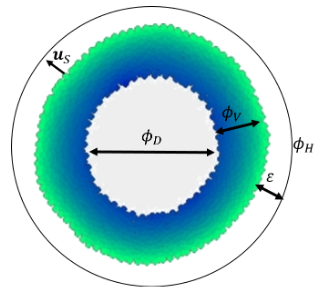
\includegraphics[width=0.5\linewidth]{modelParam.png}
    \caption{Model Parameters on a tumor cell}
    \label{fig:enter-label}
\end{figure}
\begin{itemize}
    \item $\phi_V$: volume fraction of viable tissue
    \item $\phi_D$: volume fraction of dead tissue
    \item $\phi_H$: volume fraction of healthy tissue
    \item $u_S$: tissue velocity
    \item $\varepsilon$: thickness of interface between healthy and tumoral tissue
    \item $p$: cell-to-cell (solid) pressure
    \item $n$: nutrient concentration
\end{itemize}



\section*{Equations}
\begin{equation}
    \phi_V + \phi_D + \phi_H = 1
\end{equation}
\begin{equation}
    \phi_T = \phi_V + \phi_D, \text{ where } \phi_T \text{ is the total volume fraction of tumor tissue}
\end{equation}
\begin{equation}
    \frac{\partial \phi_T}{\partial t} = M \nabla \cdot \left( \phi_T \nabla \mu \right) + S_T - \nabla \cdot \left( \phi_T u_S \right)
\end{equation}
\begin{equation}
    \frac{\partial \phi_D}{\partial t} = M \nabla \cdot \left( \phi_D \nabla p \right) + S_D - \nabla \cdot \left( \phi_D u_S \right)
\end{equation}
\begin{equation}
    \nabla \cdot \left( D(\phi_T) \nabla n \right) + T_c \left( \phi_T, n \right) - n \left( \phi_T - \phi_D \right) = 0
\end{equation}
where,
\begin{equation}
    \mu = f' \left( \phi_T \right) - \epsilon^2 \nabla^2 \phi_T
\end{equation}
\begin{equation}
    f \left( \phi \right) = \phi^2 \left( 1 - \phi \right)^2 / 2
\end{equation}
\begin{equation}
    \nabla \cdot u_S = S_T
\end{equation}
\begin{equation}
    u_S = - \kappa(\phi_T, \phi_D) (\nabla p - \frac{\gamma}{\epsilon}\nabla \phi_T)
\end{equation}
\begin{equation}
    S_T = n G \left( \phi_T \right) \phi_V - \lambda_L \phi_D
\end{equation}
\begin{equation}
    S_D = (\lambda_A + \lambda_N \mathscr{H}(n_N-n))(\phi_T - \phi_D) - \lambda_L \phi_D
\end{equation}

\section*{Discretization}
\begin{itemize}
    \item Spatial discretization: Finite Difference method
    \item Temporal discretization: Implicit Crank-Nicolson scheme
    \item Advection terms: Discretized using third-order upwind WENO approximation
    \item Laplacians and operators: Approximated to second order with averaging operators
    \item Implemented using a multigrid algorithm on a uniform mesh
\end{itemize}

The discretized equations used in the implementation are:

\begin{align}
    \phi_{T,i,j}^{k} - \phi_{T,i,j}^{k-1} &= \frac{sM}{2} \left[\nabla_d (\phi_T^k \nabla_d \mu^k)_{i,j} + \nabla_d (\phi_T^{k-1} \nabla_d \mu^{k-1})_{i,j} \right] \nonumber \\
    &\quad - \frac{s}{2} \left[\nabla_d \cdot (\mathbf{u}_S^k \phi_T^k)_{i,j} + \nabla_d \cdot (\mathbf{u}_S^{k-1} \phi_T^{k-1})_{i,j} \right] \nonumber \\
    &\quad + \frac{s}{2} \left[S_T^{k} + S_T^{k-1} \right]_{i,j} 
\end{align}

\begin{align}
    \mu_{i,j}^{k} = f'(\phi_{T,i,j}^k) - \varepsilon^2 \Delta_d \phi_{T,i,j}^k 
\end{align}

\begin{align}
    \phi_{D,i,j}^{k} - \phi_{D,i,j}^{k-1} &= \frac{sM}{2} \left[\nabla_d (\phi_T^k \nabla_d \mu^k)_{i,j} + \nabla_d (\phi_T^{k-1} \nabla_d \mu^{k-1})_{i,j} \right] \nonumber \\
    &\quad - \frac{s}{2} \left[\nabla_d \cdot (\mathbf{u}_S^k \phi_D^k)_{i,j} + \nabla_d \cdot (\mathbf{u}_S^{k-1} \phi_D^{k-1})_{i,j} \right] \nonumber \\
    &\quad + \frac{s}{2} \left[S_D^{k} + S_D^{k-1} \right]_{i,j} 
\end{align}

\begin{align}
    0 = \nabla_d \cdot \left(\kappa(\phi_T^k, \phi_D^k)_{i,j} \nabla_d p \right) + S_{T,i,j}^{k} \nonumber \\
    - \frac{\gamma}{\varepsilon} \nabla_d \cdot \left( \kappa(\phi_T^k, \phi_D^k)_{i,j} \nabla_d \phi_T^{k-1} \right) 
\end{align}

\begin{align}
    0 &= \nabla_d \cdot \left( D(\phi_T^k) \nabla_d n \right)_{i,j} + n \eta_{i,j} \left[ (\phi_{T,i,j} - \phi_{D,i,j}) + S_{C,i,j}^k \right] - n c S_{C,i,j}^k 
\end{align}

where

\begin{align}
    S_{C,i,j}^k := v_p^H (1 - Q(\phi_{T,i,j})) + v_p^T Q(\phi_{T,i,j}) 
\end{align}

\section*{Initial Conditions}
The initial condition is a slightly elliptical initial tumor.
 
\section*{Boundary Conditions}

 The model equations are valid throughout $\Omega$, and no internal boundary conditions are required for $\phi T$, $\phi D$, or any other variables. For outer-boundary conditions, we choose
$\mu = p = 0$ ,  $n = 1$, $\zeta * \Delta \phi _T = \zeta * \Delta \phi _D = 0$  on $\partial \Omega$,

 where $\zeta$ is the outward-pointing unit normal on the outer boundary $\partial \Omega$. Conditions $\mu = p = 0$ allow for the free flow of cells and water across the outer boundary to accommodate growth. 
 
\section*{References}
\begin{enumerate}
    \item Wise, S. M., Lowengrub, J. S., \& Cristini, V. (2011). An adaptive multigrid algorithm for simulating solid tumor growth using mixture models. \textit{Mathematical and Computer Modelling}, 53, 1–20.
    \item Cristini, V. \& Lowengrub, J. S. (2010). \textit{Multiscale Modeling of Cancer: An Integrated Experimental and Mathematical Approach}. Cambridge University Press.
    \item University of Oxford (2014). \textit{Cell-based Chaste: A Multiscale Computational Framework for Modelling Cell Populations}.
\end{enumerate}

\end{document}